\documentclass[twoside,10pt,twocolumn]{article}


%!TEX root = flock-comment-main.tex

%%%%% THIS IS THE SECTION WHERE THE AUTHOR PUTS IN ALL OF THEIR TITLE AND AFFILIATION
%%%%% INFORMATION AND  A FEW OTHER THINGS
\newcommand{\myTitle}{Interpreting the {\sc flock} algorithm as a statistical model}

% redefine this to make author list. Note affiliation symbols are done manually.
% All caps tends to look better
\newcommand{\myAuthors}{ ERIC C.~ANDERSON$^{*,\dagger,\S}$ and PATRICK D. BARRY$^\ddag$}

% redefine to make the affiliation list.  Note symbols are done manually
\newcommand{\myAffiliations}{$^*$Fisheries Ecology Division, 
    Southwest Fisheries Science Center, National Marine Fisheries Service, NOAA,
    110 Shaffer Road,
    Santa Cruz, CA 95060, USA, $^\dagger$Department of Applied Math and Statistics, University of
California, Santa Cruz, CA, $^\ddag$University of Alaska, Fairbanks, School of Fisheries and Ocean Science,
17101 Point Lena Loop Rd.,
Juneau, AK 99801, USA }

% the email address for the corresponding author
\newcommand{\myEmailAddress}{eric.anderson@noaa.gov}
\newcommand{\myEmailFootnote}{$^\S$}

% here you can put your very own copyright notice
\newcommand{\myCopyright}{\copyright US Federal Government work in the public domain in the USA}

% here you can put a running title (a short title that goes on the left of the 
% even pages)
\newcommand{\myRunningTitle}{A statistical perspective on {\sc flock}}

% and here you put the running author (short listing of authors for the
% upper right header on the odd pages)
\newcommand{\myRunningAuthor}{Anderson \& Barry}

%%%% DONE WITH AUTHOR/TITLE/ETC INFORMATION DEFINITION
  % Put all the author title stuff in there

% ------
% Fonts and typesetting settings
\usepackage[sc]{mathpazo}
\usepackage[T1]{fontenc}
\linespread{1.05} % Palatino needs more space between lines

\usepackage{microtype}
% ------
% Page layout
\usepackage[labelfont=bf,labelformat=simple,labelsep=quad]{caption}

\usepackage{graphicx}
\usepackage{amssymb}
\usepackage{epstopdf}
\usepackage{amsfonts}
\usepackage{natbib}
\usepackage{subfigure}
\usepackage{xspace}
\usepackage{mathrsfs}
\usepackage{fancyhdr}
\usepackage{cuted}
\usepackage{flushend}
\usepackage{color}


%% some handy things for making bold math
\def\bm#1{\mathpalette\bmstyle{#1}}
\def\bmstyle#1#2{\mbox{\boldmath$#1#2$}}
\newcommand{\thh}{^\mathrm{th}}


%% Some pretty etc.'s, etc...
\newcommand{\cf}{{\em cf.}\xspace }
\newcommand{\eg}{{\em e.g.},\xspace }
\newcommand{\ie}{{\em i.e.},\xspace }
\newcommand{\etal}{{\em et al.}\ }
\newcommand{\etc}{{\em etc.}\@\xspace}



%% the page dimensions
\textwidth = 6.5 in
\textheight = 9 in
\oddsidemargin = -0.01 in
\evensidemargin = -0.01 in
\topmargin = -0.7 in
\headheight = 0.25 in
\headsep = 0.25 in
\parskip = 0.0in
\parindent = 0.25in

\setlength{\columnsep}{.4in}


%% change section heading styles
\makeatletter
\renewcommand\section{\@startsection {section}{1}{\z@}%
                                   {-3.5ex \@plus -1ex \@minus -.2ex}%
                                   {1.5ex \@plus 0ex}%
                                   {\normalfont\normalsize\bfseries}}
\renewcommand\subsection{\@startsection{subsection}{2}{\z@}%
                                     {-3.25ex\@plus -1ex \@minus -.2ex}%
                                     {1.5ex \@plus .2ex}%
                                     {\normalfont\normalsize\itshape}}
\makeatother

%% modify the abstract environment
\renewenvironment{abstract}
{\begin{quote}{\bf Abstract}\end{quote}\begin{quote}\bfseries\small}
{\end{quote}}


\fancypagestyle{firststyle}
{
   \fancyhf{}
   \chead[]{\vspace*{.1in}
\includegraphics[width=\textwidth]{images/banner.pdf}}
   \lfoot[]{\footnotesize \myCopyright}
}

%% here is what I hope will be fancyplain
\fancyhead{} % clear all header fields
\fancyhead[LE]{{\bf \thepage}~~{\sl \myRunningTitle}}
\fancyfoot[RE,LO]{{\footnotesize \myCopyright}}
\renewcommand{\headrulewidth}{0pt}
\fancyhead[RO]{{\sl \myRunningAuthor}~~{\bf \thepage}}
\cfoot[]{}



\begin{document}


\pagestyle{fancyplain}
\thispagestyle{firststyle}



   \begin{strip}
   \mbox{}\\
   {\large\sc comment}
   \mbox{}\\
        {\LARGE\bf \myTitle \par}
    \mbox{}\\
    \uppercase{\myAuthors}\\ 
       \mbox{}\\
    {\em \myAffiliations}\\
    \mbox{}\\
    {\small \myEmailFootnote Correspondence: \myEmailAddress}
    
   \begin{abstract}
   	%!TEX root = flock-comment-main.tex

      We show that the algorithm in the program {\sc flock} \citep{Duc&Tur2009} can be
interpreted as an estimation procedure based on 
a model essentially identical to the {\sc structure} 
\citep{Pritchardetal2000} model with no admixture and non-correlated 
allele frequency priors. Rather than using MCMC, the {\sc flock} algorithm 
searches for the maximum-{\em a-posteriori}
estimate of this {\sc structure} model via a simulated 
annealing algorithm with a rapid cooling 
schedule (namely, the exponent on the objective function~$\rightarrow \infty$).  We 
demonstrate the similarities between the two programs in a two step approach. First,
to enable rapid batch processing of many simulated data sets,
we modified the source code of  {\sc structure} to use the {\sc flock} algorithm, producing
the program {\sc flockture}. With simulated data we confirmed that results obtained with
{\sc flock}  and {\sc flockture} are very similar (though flockture is some 200 times faster). 
Second, we simulated multiple large data sets under varying 
levels of population differentiation for both microsatellite and SNP genotypes. We analyzed them
with {\sc flockture} and {\sc structure} and assessed each program on its ability to cluster
individuals to their correct subpopulation.  We show that
{\sc flockture} yields results similar to {\sc structure} albeit with greater 
variability from run to run. {\sc flockture} did perform better than {\sc structure} 
when genotypes were composed of SNPs and differentiation was moderate 
($F_{ST}=0.022-0.032$). When differentiation was low, {\sc structure} outperformed {\sc flockture}
for both marker types. On large data sets like those we simulated, it appears that 
{\sc flock}'s reliance on inference rules regarding its ``plateau record'' are not helpful. 
Interpreting {\sc flock}'s algorithm as a special case of the model in 
{\sc structure} should aid in understanding the program's output and behavior. 

    %% Put abstract text in here
    \end{abstract}
   \end{strip}


%!TEX root = flock-comment-main.tex

\section*{Introduction}
In most fields, proposed methods that are 
perceived to be fundamentally novel or new garner more
attention and accolades---and have a higher chance of 
publication---than methods that are clearly minor elaborations upon existing work. 
Not surprisingly, then, in articles and manuscripts, authors may 
emphasize the differences and downplay the similarities between their 
work and the published literature.   In molecular ecology, this 
tendency amongst the creators of statistical methodology can make it 
difficult for end-users to understand the relationship between 
different methods.

Of course, new methods almost always build upon pre-existing ones, and 
much is to be gained by understanding the close relationship between 
different statistical methods in use in molecular ecology today.  
Indeed, some authors downplay the similarities between their method and 
existing ones not because they wish to make their method seem more 
novel, but rather because they are genuinely unaware of the close ties 
between their work and existing methods.  Identifying the 
similarities between new and existing work should help our field
by 1) reducing end-user confusion about whether 
it is necessary to analyze data with a (sometimes overwhelming) variety 
of computer programs; 2) establishing a common language upon which to 
compare different methods; and 3) providing a principled perspective 
from which to argue about the expected strengths and weaknesses of any 
method.

Methods for the unsupervised clustering of genotypes have received 
considerable attention in the molecular ecology literature.  
The best known example of this class of methods is {\sc structure} 
\citep{Pritchardetal2000}.  {\sc structure} itself can be described 
as an elaboration of earlier models used to identify the spawning 
stock of salmon \citep{Smouseetal1990}, and a variety of other 
clustering methods have been developed that are all closely related to 
{\sc structure}, for example {\sc NewHybrids} \citep{And&Tho2002}, {\sc 
BayesAss+} \citep{Wil&Ran2003}, and {\sc baps} 
\citep{Coranderetal2004}. An overview of these similarities can be 
found in \citet{Anderson2009PGAC}.

Recently, a description of the software {\sc flock} was published, 
billing the method as a ``non-Bayesian method [that] 
differs substantially from previous 
clustering algorithms'' \citep[][p.~1333]{Duc&Tur2009}. A following
paper asserts that
\begin{quote}
``{\sc flock} is very different from  other clustering 
programs. It does not sample the space of partitions through small 
random step walks as in MCMC, and it does not try to optimize some 
target function, such as HWLE\@. Briefly stated, it is not based on a 
probabilistic search algorithm. On the contrary, {\sc flock} is 
entirely deterministic'' \citep[][p.~736]{Duc&Tur2012}.
\end{quote}
These papers describe the rationale behind the {\sc flock} algorithm in
intuitive terms with analogies to the coalescence of flocks of birds
or the accretion of snow on a moving snowball, \etc  

Here, we provide a different perspective on the {\sc flock} algorithm,
showing it to be a special, restricted case of the simulated annealing
algorithm for finding the Bayesian maximum {\em a posteriori}
estimate from a marginalized form of the {\sc structure} model with no
admixture and non-correlated allele frequencies.  For illustration, we subsequently compare
the results obtained from {\sc flock} and {\sc structure} on a real data
set with $>$2,500 individuals.

\section*{Comparison of methods}
We start with a succinct mathematical description of the {\sc structure}
model, then describe the {\sc flock} algorithm, and finally explain
the close relationship between the two.


\subsection*{{\sc structure}}
In the {\sc structure} model with no admixture, the unknown ``subpopulation'' that the 
$i\thh$ individual ($i=1,\ldots,N)$ belongs to is denoted by $Z_i \in \{1,\ldots,K\}$, 
where $K$ is the 
number of subpopulations (or clusters, as they are often referred to).  
In a diploid individual from cluster $k$, the 
allelic types of the two gene copies at the $\ell\thh$ locus are assumed
to be drawn independently from the vector of allele frequencies at
locus $\ell$ in subpopulation $k$,  $\theta_{k\ell}=(\theta_{k\ell 1},\ldots,\theta_{k\ell A_\ell})$, where 
$A_\ell$ 
denotes the number of alleles observed in the data set at locus $\ell$.
Hence, if $Y_{i\ell}$ denotes a vector of length $A_\ell$ whose components denote the 
number
of copies of each of the $A_\ell$ alleles at locus $\ell$ in individual $i$, and 
$Z_i=k$, then $Y_{i\ell}$ follows the multinomial distribution of two trials with
$A_\ell$  components and cell probabilities given by the allele frequencies: 
\begin{equation}
(Y_{i\ell}~|~Z_i=k) \sim \mathrm{Mult}_{A_\ell}(2, \theta_{k\ell}).
\end{equation}
In the {\sc structure} model without physical linkage, the genotypes at the loci are assumed to
be independent of one another, so the probability of the genotype data at
all $L$ loci---$Y_i=(Y_{i1},\ldots,Y_{iL})$---is simply a product of multinomial 
probabilities.
In the uncorrelated allele frequencies model, the prior on each $\theta_{k\ell}$ is a
Dirichlet distribution with parameters $(\lambda_{k\ell1},\ldots,\lambda_{k\ell A_
\ell})$,
which are usually all set to a value such as 1 or $1/A_\ell$.  

After initializing the unknown allele frequencies, $\theta = (\theta_1,\ldots,\theta_K)$, to randomly drawn values,
$\theta^{(0)}$, inference in the model proceeds by sampling from the joint posterior of the 
$Z_i$'s and $\theta$ using Gibbs sampling.  That is,
at iteration $t = 0, 1, 2, \ldots$:
\begin{enumerate}
\item each $Z^{(t)}_i$ is updated to $Z^{(t+1)}_i$ by sampling a value from 
the full conditional distribution of $Z_i$ given
$Y_i$ and $\theta^{(t)}$ (the current estimate of the allele frequencies).  This
distribution is found using Bayes' theorem. In {\sc structure}'s formulation, the 
prior probability that $Z_i=k$ is $1/K$ for all $k=1,\ldots, K$.     
\item $\theta^{(t)}$ is updated to $\theta^{(t+1)}$ from its full conditional distribution.  For each 
cluster
$k$ and locus $\ell$, the full conditional for $\theta_{k\ell}$ is independently a 
Dirichlet distribution with parameters $\lambda_{k\ell j} + \#(k,\ell,j)$, for 
$j=1,\ldots, A_\ell$,
where $\#(k,\ell,j)$ is the number of alleles of type $j$ at locus $\ell$ observed in 
individuals with $Z^{(t+1)}_i = k$.   
\end{enumerate}

It will be useful for our comparison with {\sc flock} to point out that another way 
of pursuing inference in this model would be to first integrate out the 
Dirichlet priors on the allele frequencies and then sample from the posterior
for the $Z_i$'s by Gibbs sampling.  When $\theta$ is integrated out, the genotypes 
of the individuals are no longer conditionally independent (they were originally
independent {\em conditional} on $\theta$ and the $Z_i$'s), so the calculation of 
the full conditional distribution of $Z_i$ becomes somewhat more involved,
but can be computed by the following reasoning. First, the full 
conditional distribution of $Y_{i\ell}$, given that individual $i$ is from subpopulation $k$
(\ie $Z_i=k$), depends on the 
cluster memberships and genotypes  of all the remaining individuals,
which we denote by  $Z_{(-i)}$ and $Y_{(-i)\ell}$, respectively.
This full conditional for $Y_{i\ell}$ follows 
a Compound Dirichlet Multinomial distribution (CDM):
\begin{eqnarray}
\lefteqn{(Y_{i\ell}~|~Z_i=k,~Z_{(-i)},~Y_{(-i)\ell}) \sim} \label{eq:cdm}\\
& & \mathrm{CDM}(\lambda_{k\ell 1} + \#_{(-i)}(k,\ell,1), \ldots,
\lambda_{k\ell A_\ell} + \#_{(-i)}(k,\ell,A_\ell)), \nonumber
\end{eqnarray}
where $\#_{(-i)}(k,\ell,j)$ is the number of alleles of type $j$ at locus $\ell$
found in individuals {\em other than individual $i$} that currently
belong to cluster $k$. Thus, calculating (\ref{eq:cdm}) for each value of $Z_i=k \in 
\{1,\ldots,K\}$ 
and normalizing to sum to one gives the full conditional distribution for 
$Z_i$:
\begin{equation}
P(Z_i=k~|~Y_i, ~Z_{(-i)},~Y_{(-i)\ell})~~,~~k=1,\ldots,K.
\label{eq:fc}
\end{equation}
A new value of $Z_i$ would be drawn from (\ref{eq:fc}) if doing Gibbs sampling in this
version of the {\sc structure} model in which $\theta$ has been integrated out.  In 
fact,
this is the approach (with a slightly different prior weight on the $Z_i$'s) taken to 
update 
$Z_i$ in both {\sc hwler} \citep{Pel&Mas2006} and {\sc structurama} \cite{Hue&And2007} 
when not
proposing changes to the number of clusters.



\subsection*{{\sc flock}}
Here we translate the recipe given by \citeauthor{Duc&Tur2009} for the 
{\sc flock} algorithm into a specification in terms of the variables
defined in the previous section.  We provide the description for a case in which
it is assumed there are $K$ clusters.

The first step of the flock algorithm is initialization, during which 
the program randomly allocates each of the $N$ individuals to one of 
$K$ clusters.  Then a number of reallocation steps are performed.  During every one of 
these steps, each individual is given the chance to be reallocated 
(\ie moved to a different cluster).  This is done on the basis of 
maximum likelihood: as \citeauthor{Duc&Tur2009} say (2009, p.~1335), ``Re-allocations are 
performed following multilocus maximum likelihood (Paetkau et al. 1995).''

From that description, it is not clear how \citeauthor{Duc&Tur2009} treat 
alleles that appear in the focal
individual but do not appear within any other individuals within a cluster.
The original approach of \citet{Paetkauetal1995} merely added 0.01 or some other
small value to each allele frequency that was 0, and then renormalized 
the allele frequencies to sum to 1.  In later works, Paetkau and colleagues
also employed the ``Bayesian'' approach of \citet{Ran&Mou1997} in their 
software {\sc geneclass2}  \citep{Piryetal2004}.  If \citeauthor{Duc&Tur2009}
use the approach of \citet{Ran&Mou1997}, then the $i\thh$ individual will
be reallocated to whichever cluster gives the highest value to 
$P(Y_{i\ell}~|~Z_i=k,~Z_{(-i)},~Y_{(-i)\ell})$, which is exactly the probability
defined in (\ref{eq:cdm}).  
If \citeauthor{Duc&Tur2009} use the simpler ``add 0.01 and renormalize''
formulation of \citet{Paetkauetal1995}, then their reallocations are based
on maximizing a likelihood that, although it may not be formally identical to
that in (\ref{eq:cdm}), is nearly identical to it.   

It is worth pointing out that, since the
{\sc structure} model without admixture assumes a uniform prior over 
the $K$ different clusters, $P(Y_{i\ell}~|~Z_i=k,~Z_{(-i)},~Y_{(-i)\ell})$
is exactly proportional to $P(Z_i=k~|~Y_i, ~Z_{(-i)},~Y_{(-i)\ell})$, which 
we have shown is the
full conditional distribution for $Z_i$ in the {\sc structure} model after
integrating out $\theta$.  Thus, we have shown that, doing Gibbs
sampling for $Z_i$ in  the {\sc structure} in which $\theta$ has been
integrated out would involve sampling a new value of $Z_i$ from the 
probability distribution,
\[
P(Z_i=k~|~Y_i, ~Z_{(-i)},~Y_{(-i)\ell})
\]
and that the updates that
{\sc flock} makes to each $Z_i$ involve assigning to $Z_i$
\begin{equation}
\arg\max_k P(Z_i=k~|~Y_i, ~Z_{(-i)},~Y_{(-i)\ell}),
\end{equation}
\ie the value of $k$ that maximizes $P(Z_i=k~|~Y_i, ~Z_{(-i)},~Y_{(-i)\ell})$
(or, as stated above, a nearly identical function of $k$, depending on how
the program {\sc flock} treats alleles that are not observed in certain clusters).






\subsection*{{\sc flock} as a special case of {\sc structure}}
The goal of {\sc structure}'s MCMC algorithm is to sample from the space of 
$Z$'s in proportion to their posterior probability.  If, all that was desired
was a point estimate of the $Z_i$'s that maximized the posterior probability,
then one standard approach to finding that maximimum {\em a posteriori}, or MAP, 
estimate, would be to use simulated annealing \citep{Kirkpatricketal1983}.
To do simulated annealing in the {\sc structure} model with no admixture and
no correlated allele frequency prior, after integrating out the unknown
allele frequencies, the updates for each $Z_i$ would be made from the 
distribution
\[
\biggl[P(Z_i=k~|~Y_i, ~Z_{(-i)},~Y_{(-i)\ell})\biggr]^\beta
\]
which is the same full conditional distribution as the marginalized {\sc structure}
model (equation~\ref{eq:fc}), raised
to the power $\beta$.  In typical applications of simulated annealing,
$\beta$ is set to a starting value less than 1, and, as the algorithm proceeds,
$\beta$ is increased according to a ``cooling schedule''\citep{Hajek1988}, until
the algorithm finds a local maximum in the posterior probability surface.  
When $\beta$ is small, the process can easily traverse ``valleys''
in the posterior probability surface and has a better chance of searching
more of the space for the maximum value.  As $\beta$ gets larger, it becomes
more probable that the process will
move uphill on the probability surface, tending toward the local
maximum near where it currently is.    

It should now be clear that the algorithm in {\sc flock} is a simulated annealing 
algorithm for the {\sc structure} model in which the cooling schedule is
``start with $\beta\rightarrow\infty$ and leave it there for the duration of 
the algorithm.''  As such, we can expect that it may not provide the best 
mechanism for searching for the MAP estimate and it may be more susceptible 
to becoming trapped in local modes of the posterior probability. 
In the following section we show that {\sc structure} and {\sc flock} find similar
solutions in the analysis of a large microsatellite data set, though, as expected,
{\sc flock} seems to find the same solution less consistently than does {\sc structure}.





\section*{Performance Comparison with {\sc structure}}

\subsection*{Analysis of coastal California steelhead} 
To compare the behavior of {\sc flock} to that of {\sc structure} we used a published 
dataset of 2596 steelhead \textit{Oncorhynchus mykiss}
genotyped at 15 microsatellite loci from \citet{Garzaetal_norcal}.  {\sc flock} was run six times using the default setting for all 
run parameters (initial partition = random, number of iterations = 20, number of runs = 50, 
LLOD threshold = 0) for values of $K$ from 2 to 6. The stopping point of 
$K=6$ was chosen after four consecutive runs (at $K=6$) % <-- Patrick, is that right. were the non-plateau-ing runs at K=6?
yielded no plateau (see below). For each value of $K$ from 2 to 6, the no-admixture, 
uncorrelated-allele-frequency model implemented in {\sc structure} was run 6 times using 
50,000 sweeps of burn-in followed by 150,000 sweeps of sample collection from the posterior. 
All runs were performed on a (WHAT TYPE OF COMPUTER?) with an i7 3.40GHz processor and 8GB
of RAM. To facilitate the comparison of results from
the two programs, we derived $q_i$ values 
from {\sc flock}'s output by exponentiating the log-likelihood values for cluster membership  % <-- Patrick, please verify.
and rescaling so they summed to one.  These are then comparable to the $q_i$ values
returned by {\sc structure}, which, in the no-admixture case, are posterior probabilities of cluster membership.
The program {\sc clumpp} \citep{Jak&Ros2007} was used to relabel clusters among different runs,
while the program {\sc district} \citep{Rosenberg2004} was used to plot individual \textit{$q_i$} values. 

\citet{Duc&Tur2012} promote a method for using {\sc flock} to estimate, $K$, the number of
subpopulations.  Their approach involves INSERT SHORT DESCRIPTION, INCLUDING DISCUSSION OF PLATEAUS.

It is now common practice to use the approximate marginal likelihood ($\ln P(D)$) from {\sc structure}
or a derived quantity such as $\Delta K$ \citep{Evannoetal2005} to try to estimate $K$.
While we take the stance that estimates of $K$ made with {\em any} unsupervised clustering algorithm
from data on real (non-idealized) populations should always be interpreted and used
cautiously, it is nonetheless instructive to compare \citet{Duc&Tur2012}'s method for
estimating $K$ to results obtained using $\ln P(D)$ and $\Delta K$, and we do so. 


\subsection*{Results} 
Run times were relatively short for both programs. {\sc flock} 
required 1133 minutes to complete all the runs, averaging 188.8 minutes for 
each of six groups of runs over $K$ from 2 to 6. {\sc structure} completed all the runs in 
486 minutes with each of the six groups of runs averaging 80.8 minutes. Increasing
$K$ from of 2 to 6 increased {\sc flock}'s run time by a factor of 2.4, but {\sc structure}'s
run time was increased by a factor of only 1.6.  
\hrule

The allocation of indivividuals into K clusters was congruent for each program. For all six groups 
of runs from \textit{k}=2-4, {\sc flock} lead to nearly identical clustering of individuals 
(See supplementary materials). It should be noted
that of the 50 starting allocations of individuals in the {\sc flock} procedure likelihoods of each individual in 
each reference is only reported for the 
 'best run'. Of these 'best runs' for a \textit{k} of 2 only two  
ended with identical clustering (same mean LLOD score), all other runs 
differed by at most the allocation of 13 individuals. As \textit{k} increases so do the number of solutions
that {\sc flock} finds (Fig 1). These solutions, however, are suprisingly similar to
 the partions identified by {\sc structure}. Both programs idenfity clusters 
which can be attributed to the geographical boundaries identified by \citet{Garzaetal_norcal}.

Despite the similar allocation of individuals into \textit{k} clusters, the 
plateau analysis in {\sc flock} leads to different conclusions among groups of runs, as well as 
one that differs from {\sc structure}. While no plateaus were observed in any of the six groups 
for a \textit{k} $\geq$2, the plateau record varied greatly among each
 group for \textit{k}=2 (plateau  sequences- Run1= 3,2,3,7,4; Run2=2,5,2,3,2,3; Run3=2,2,2,2,2,5; 
Run4=2,3,4,2,4,3; Run5=2,2,5,5,3; and; Run6=2,2,2,2,2,3,3). The plateau analysis 
procedure suggested by \citet{Duc&Tur2012} leads to 
either an estimate of K$\geq$2 (Run1) or \textit{undecided} as a consequence of no plateau 
lengths being greater than 6. Interpreting the results from {\sc structure} is often accomplished by 
looking at the estimated log likelihood of the data given K, the delta k method \citep{Evannoetal2005}, and plots of 
individual \textit{$q_i$} values. Both the estimated likelihood of the data
and the plots of individuals \textit{$q_i$} values suggest that 
the most likely \textit{k} for the dataset is 6. 

\begin{figure*}
\begin{center}
	 % NOTE. Eric made Flock-Fig1.jpg as a Preview because Flock-Fig1.pdf
	 % ate up too many resources while editing the document.  For final 
	 % production, it should be changed back to Flock-Fig1.pdf
    \includegraphics[width=\textwidth]{images/Figures-Pat/Flock-Fig1-GreyScale.pdf} % Flock-Fig1.jpg}  
    \caption{Assignment to reference population (from \textit{k} = 2-6) plots created 
in the program {\sc flock}. Each horizontal plot represents the 'best run' from a 
series where individuals are reallocated into \textit{k} clusters. Within each plot 
the normalized individual likelihood for each reference population is represented by a 
colored vertical bar. Major geographic boundaries that were attributed to genetic 
structure in \citet{Garzaetal_norcal} are indicated with black vertical lines. Results 
from the 'best runs' showed similar geographic differentiation to 
\citet{Garzaetal_norcal} analysis. The plateau analysis developed by 
\citet{Duc&Tur2012} indicate that either an undecided structure or that \textit{k}=2 
is the lower bound estimate.}
    \label{Fig.1}
\end{center}
\end{figure*}

\begin{figure*}
\begin{center}
	% NOTE. Pat made Q-val-StrFloc.pdf that has all runs individually, replaced with 
	% all of them on same axis. It will look fine as a black and white with different 
	% characters.
 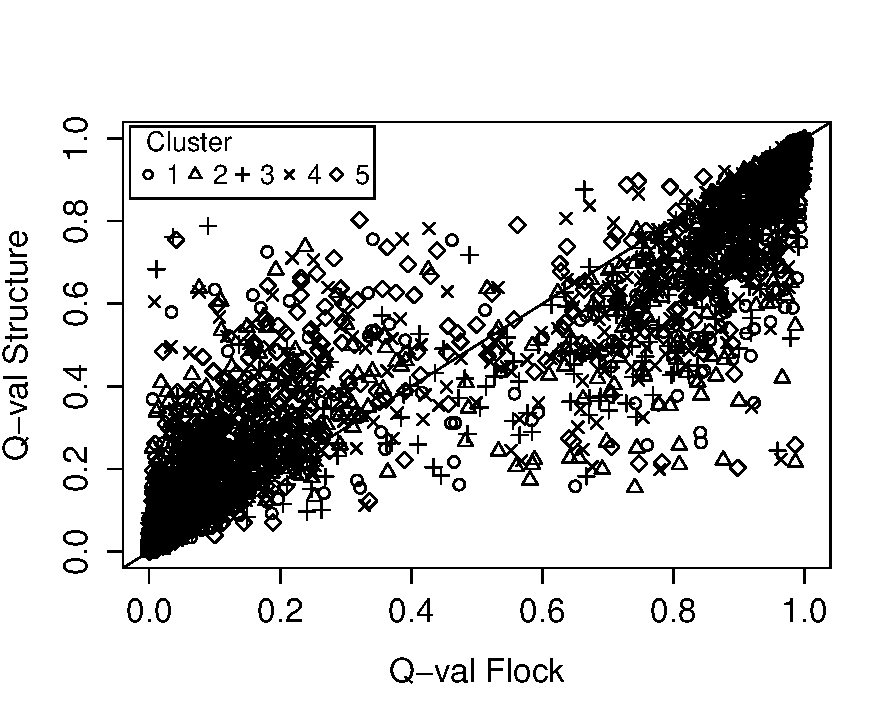
\includegraphics[width=\textwidth]{images/Figures-Pat/Qval-1plotGreyScale.pdf}
    \caption{Individual \textit{$q_i$} values plotted for each cluster for \textit{k}=5. 
{\sc flock} estimates of likelihood of assignment to each cluster have less uncertainty
 attributed to them.}
    \label{Fig.2}
\end{center}
\end{figure*}


To investigate the ability of the arrangement of individuals within the reference 
populations to move around the partition space we varied the number of iterations that 
each run goes through to find the 'optimal' allocation of individuals. Unfortuantely 
only the reallocation matrix for the 'best run' is given as output. Increasing the 
number of iterations did not affect the overall inference of \textit{k}. It was 
observed that often during the last iterations individuals would alternate between 
reference groups during subsequent iterations. Increasing the log likelihood 
difference threshold for reallocation to 0.18 (there needs to be at least a 1.5 times 
higher likelihood to reallocate the individual) minimized this, but did not affect the 
inference of \textit{k} (lower bound estimate of \textit{k} = 2). 


\section*{Conclusions}

One of the major claimed advantages of {\sc flock} over MCMC methods for solving the 
K-partition problem is that, '[t]he very short processing times for each run of {\sc flock} allows for
 comparing partitions from many runs of each \textit{k}'' \citep[][p.~735]{Duc&Tur2012}.
While the authors observed improved process time in their 
comparisions we did not observe the same advantage in our analysis. In their comparison, the 
run parameters for {\sc flock} were 50 runs and 20 iterations for each \textit{k} = 1 to K+4. 
These process times were compared to the admixture model with correlated allele 
frequencies in {\sc structure} with ten iterations of a 50,000 sweep burn-in followed 
by 200,000 sweep sample from the posterior of \textit{k} from 1 to K+3. 
It seems reasonable, for each \textit{k}, to compare one iteration of {\sc structure} 
to one iteration of {\sc flock} with 50 different starting allocations that are reallocated 20 times 
as both evaluate the partition space once. Process speed advantages also may only been observed 
with low sample sizes. The authors evaluated simulated data sets with sample sizes of N = 60, 120, 
and 240. 

The partition space over which {\sc flock} evaluates how individuals are clustered 
greatly increases with both the number of individuals and the number of clusters into 
which they can be partitioned. The total partition space for any given k can be 
defined by $\sum\limits_{i=1}^k S(n,k)$ where S(n,k) is a Stirling number of the 
second kind. The results of {\sc flock} depend primarily on the initial partition of 
individuals. It is not surprising that with 2,596 individuals we could have 
drastically different plateau sequences with just two clusters and that as \textit{k} increases
{\sc flock} finds suboptimal allocations. 

For those that do decide to use {\sc flock} as an alternative to {\sc structure}, the adhoc rules 
to estimate K may be overly stringent. While there has been ample 
discourse concering choosing the optimal K in  {\sc structure} \citep{Evannoetal2005, 
Prichardetal2000, Wap&Gag2006} and \citet{Pritchardetal2000} urges users 
to be cautious of interpreting K, no such care in interpreting results 
is suggested in running {\sc flock}. The authors developed estimation rules based on simulated data 
sets with different migration regimes and rates, number of loci, and K. 
By relying on identical allocations (mean LLOD values) as a means of supporting 
a particular \textit{k},  similar but not idential 
allocations will provide no support to a given \textit{k}. This may not be as big an issue with small datasets,
however, as sample sizes increase this could have a drastic influence on the estimation of 
K. 



 


\bibliographystyle{men}
{\footnotesize
\bibliography{flock-comment}}

 \end{document}


